\section{Dreaming with the Animals}

\begin{quotex}
Now the animal man receiveth not the things of the Spirit of God: for they are foolishness unto him; and he cannot know them, because they are but spiritually judged. But he that is spiritual, on the contrary, judgeth all things, and he himself is judged by no man. \flright{\textsc{I Corinthians ii: 14-15}}

\end{quotex}

There are four kingdoms or realms of Nature: the mineral, plant, animal and human. The human realm incorporates all four realms in its being. The mineral realm was dealt with in \textit{The Hour of the Morning Star}\footnote{\url{https://gornahoor.net/?p=15116}}. The plant realm, or Etheric Soul, was described in \textit{Sex and Tropism}\footnote{\url{https://gornahoor.net/?8349}}. The properties of the rational soul, which is properly human, will follow up on this one.

The animal, or astral, soul is the seat of feelings and emotions, both positive and negative. It also produces the imagery of the world. The external world is active in regard to the animal soul. That is, the world dominates the animal soul, creating a representation of itself in the soul of the animal. Hence the soul is passive in relation to the world; there is no escaping it.

\begin{wrapfigure}{er}{.4\textwidth}
 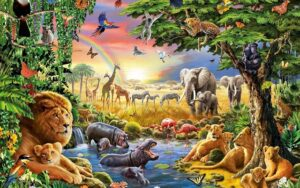
\includegraphics[scale=.55]{a20211024DreamingwiththeAnimals-img001.jpg} 
 \caption{Animal Dreams}
\end{wrapfigure}

Similarly, the animal has an inner world of its desires and emotions. The primary motivations are fear, sex, and hunger, although there are more positive emotions like playfulness, affection, pleasure-seeking, etc. Likewise, the soul is passive in relation to the inner forces. The animal experiences fear, sex, and hunger directly without mediation. Although the animal can choose, its choices are not free; rather, they are driven but its emotions.

Hence, animals exist in a dream-like state. In dreams, we are passive to the flow of the dream (barring unusual experiences like lucid dreaming). To understand the animal soul, imagine sensations and emotions without thought. When a desire arises, imagine immediately acting on it. Obviously, there can be conflicting drives. For example, hunger may arise, but fear makes the animal cautious.

Because an animal does not have knowledge of essences, every experience is novel. You see that  in young children who say ``again, again!" whenever they enjoy a game. Eventually they get bored. Your dog, on the other hand, never gets bored about jumping up for a treat. Even adults, moreover, can find themselves in the mode of repeating the same experiences over and over. Unfortunately, such beings are often centered in their animal soul.

The boundaries between the etheric body, animal soul, and rational soul are not hard, but rather merge into each other. For example, the animal soul does share in the intelligence of the rational soul. However, since it remains part of the animal soul, it cannot dominate or master the animal soul. Only the fully human rational soul can do so.



\flrightit{Posted on 2021-10-24 by Cologero }
